\documentclass[aps,prapplied,reprint,longbibliography]{revtex4-2}

\usepackage{amsmath,amssymb,amsfonts}
\usepackage{graphicx}
\usepackage{booktabs}
\usepackage{xcolor}
\usepackage[hidelinks]{hyperref}

% Generated deterministically by generate_wp2_paper_assets.py -- do not edit by hand.
\newcommand{\WpFezJobId}{dc1tqvinj2vs73dfrts0}
\newcommand{\WpFezBackend}{ibm\_fez}
\newcommand{\WpFezQubits}{27}
\newcommand{\WpFezEdges}{26}
\newcommand{\WpFezBlocks}{4}
\newcommand{\WpFezPubsPerBlock}{12}
\newcommand{\WpFezTotalPubs}{48}
\newcommand{\WpFezShotsPerPub}{2{,}048}
\newcommand{\WpFezTotalShots}{98{,}304}
\newcommand{\WpFezPooledShots}{8{,}192}
\newcommand{\WpFezCzCount}{52}
\newcommand{\WpFezSxCount}{378}
\newcommand{\WpFezQpuSeconds}{28}
\newcommand{\WpKonigSizes}{10, 10, \text{and } 6}
\newcommand{\WpCalMeanRoPct}{0.93}
\newcommand{\WpCalMaxRoPct}{1.86}
\newcommand{\WpEmpMeanRoPct}{1.14}
\newcommand{\WpEmpMaxRoPct}{4.13}
\newcommand{\WpHiddenRoFaults}{0}
\newcommand{\WpLayoutList}{114, 115, 99, 95, 94, 93, 79, 92, 91, 90, 98, 111, 110, 109, 118, 112, 108, 89, 88, 78, 69, 68, 70, 71, 58, 73, 74}
\newcommand{\WpSinkhornEps}{0.05}
\newcommand{\WpEqSevenUnifTwentySeven}{0.50918}
\newcommand{\WpThetaOne}{2.118}
\newcommand{\WpThetaStar}{2.618}
\newcommand{\WpThetaThree}{3.118}
\newcommand{\WpArmAEntOne}{12.78}
\newcommand{\WpArmAEntStar}{12.98}
\newcommand{\WpArmAEntThree}{13.00}
\newcommand{\WpArmAUniqOne}{7{,}432}
\newcommand{\WpArmAUniqStar}{8{,}131}
\newcommand{\WpArmAUniqThree}{8{,}187}
\newcommand{\WpArmAEqSevenWOne}{0.3266}
\newcommand{\WpArmAEqSevenWStar}{0.4106}
\newcommand{\WpArmAEqSevenWThree}{0.4483}
\newcommand{\WpArmAEqSevenROne}{0.6734}
\newcommand{\WpArmAEqSevenRStar}{0.5894}
\newcommand{\WpArmAEqSevenRThree}{0.5517}
\newcommand{\WpArmARawWOne}{0.1241}
\newcommand{\WpArmARawWStar}{0.1725}
\newcommand{\WpArmARawWThree}{0.1904}
\newcommand{\WpArmARawROne}{0.8759}
\newcommand{\WpArmARawRStar}{0.8275}
\newcommand{\WpArmARawRThree}{0.8096}
\newcommand{\WpArmADebSkOne}{+0.000010}
\newcommand{\WpArmADebSkStar}{-0.000019}
\newcommand{\WpArmADebSkThree}{+0.000001}
\newcommand{\WpArmADebLpOne}{+0.000512}
\newcommand{\WpArmADebLpStar}{-0.000001}
\newcommand{\WpArmADebLpThree}{+0.000365}
\newcommand{\WpArmBEqSevenWOne}{0.4571}
\newcommand{\WpArmBEqSevenWStar}{0.4786}
\newcommand{\WpArmBEqSevenWThree}{0.4856}
\newcommand{\WpArmBRawWOne}{0.1877}
\newcommand{\WpArmBRawWStar}{0.2037}
\newcommand{\WpArmBRawWThree}{0.2118}
\newcommand{\WpArmBDebSkOne}{+0.000051}
\newcommand{\WpArmBDebSkStar}{-0.000076}
\newcommand{\WpArmBDebSkThree}{-0.000066}
\newcommand{\WpHOneThreshold}{0.005}
\newcommand{\WpHOneMaxAbs}{0.000076}
\newcommand{\WpDeltaSmall}{0.20}
\newcommand{\WpDeltaLarge}{0.45}
\newcommand{\WpSigmaThreshold}{10}
\newcommand{\WpDriftNullMean}{+0.000005}
\newcommand{\WpDriftNullSe}{0.000021}
\newcommand{\WpDriftSmallMean}{+0.000972}
\newcommand{\WpDriftSmallSe}{0.000083}
\newcommand{\WpDriftLargeMean}{+0.003444}
\newcommand{\WpDriftLargeSe}{0.000249}
\newcommand{\WpDriftLargeZ}{13.76}
\newcommand{\WpFezSweepRows}{Arm A (\texttt{NB11\_REPAIRED}) & 2.118 & 7{,}432 & 12.78 & 0.3266 & 0.1241 & 0.0895 & +0.000512 & +0.000010\\
Arm A (\texttt{NB11\_REPAIRED}) & 2.618 & 8{,}131 & 12.98 & 0.4106 & 0.1725 & 0.1340 & -0.000001 & -0.000019\\
Arm A (\texttt{NB11\_REPAIRED}) & 3.118 & 8{,}187 & 13.00 & 0.4483 & 0.1904 & 0.1540 & +0.000365 & +0.000001\\
\addlinespace
Arm B (\texttt{BRICKWALL}) & 2.118 & 8{,}176 & 13.00 & 0.4571 & 0.1877 & 0.1563 & -0.000249 & +0.000051\\
Arm B (\texttt{BRICKWALL}) & 2.618 & 8{,}185 & 13.00 & 0.4786 & 0.2037 & 0.1698 & +0.000570 & -0.000076\\
Arm B (\texttt{BRICKWALL}) & 3.118 & 8{,}191 & 13.00 & 0.4856 & 0.2118 & 0.1751 & -0.000878 & -0.000066\\}
\newcommand{\WpSimShots}{512}
\newcommand{\WpSimNullThreshold}{0.002}
\newcommand{\WpSimMaxAbsMatchedSk}{0.000075}
\newcommand{\WpSimMaxAbsMatchedLp}{0.000402}
\newcommand{\WpSimMinDriftZ}{14.10}
\newcommand{\WpUnifNinetySixRawLp}{0.12482}
\newcommand{\WpUnifNinetySixRawZ}{855.48}
\newcommand{\WpUnifNinetySixDebLp}{+0.000187}
\newcommand{\WpUnifNinetySixDebSk}{-0.000018}
\newcommand{\WpUnifNinetySixDebSkZ}{-0.34}
\newcommand{\WpDriftAndSimRows}{\texttt{SIM} 27Q \texttt{NB-11} ($\theta=2.618,\,\epsilon=0.00$) & 27 & 21.90 & 0.03369 & +0.000154 & -0.000043 & -0.76\\
\texttt{SIM} 27Q \texttt{NB-11} ($\theta=3.118,\,\epsilon=0.00$) & 27 & 26.99 & 0.05287 & +0.000086 & +0.000014 & +0.17\\
\texttt{SIM} 27Q \texttt{NB-11} ($\theta=2.618,\,\epsilon=0.05$) & 27 & 21.90 & 0.04654 & +0.006140 & +0.006305 & +31.98\\
\texttt{SIM} 50Q \texttt{H2-1} ($\theta=3.118,\,\epsilon=0.00$) & 50 & 49.98 & 0.08929 & +0.000402 & +0.000019 & +0.23\\
\texttt{SIM} 50Q \texttt{H2-1} ($\theta=2.618,\,\epsilon=0.05$) & 50 & 40.56 & 0.08124 & +0.008101 & +0.008676 & +43.00\\
\texttt{SIM} 96Q \texttt{Helios-1} ($\theta=3.118,\,\epsilon=0.00$) & 96 & 95.96 & 0.12469 & -0.000046 & +0.000016 & +0.33\\
\texttt{SIM} 96Q \texttt{Helios-1} ($\theta=2.618,\,\epsilon=0.05$) & 96 & 77.88 & 0.11358 & +0.006453 & +0.006287 & +73.64\\
\texttt{SIM} $\mathrm{Unif}(\{0,1\}^{96})$ null & 96 & 96.00 & 0.12482 & +0.000187 & -0.000018 & -0.34\\
\addlinespace
\texttt{HW} \texttt{ibm\_fez} Arm B A/A ($\Delta\theta=0$) & 27 & 13.00 & -- & -- & +0.000005 & +0.24\\
\texttt{HW} \texttt{ibm\_fez} Arm B ($\Delta\theta=0.20$) & 27 & -- & -- & -- & +0.000972 & +11.71\\
\texttt{HW} \texttt{ibm\_fez} Arm B ($\Delta\theta=0.45$) & 27 & -- & -- & -- & +0.003444 & +13.76\\}
\newcommand{\WpMarrJobId}{dau0q3qhcrkc73durtgg}
\newcommand{\WpMarrQubits}{8}
\newcommand{\WpMarrCircuits}{20}
\newcommand{\WpMarrTotalShots}{10{,}240}
\newcommand{\WpQecJobId}{dbtl2vb2kf8s73c9a0d0}
\newcommand{\WpQecCircuits}{192}
\newcommand{\WpQecTotalShots}{393{,}216}
\newcommand{\WpMarrMaxAaAbsSk}{0.000407}
\newcommand{\WpMarrMaxAaEqSeven}{0.2334}
\newcommand{\WpMarrSixteenStagNoneSk}{0.08531}
\newcommand{\WpMarrSixteenStagPairSk}{+0.000042}
\newcommand{\WpMarrThirtyTwoStagNoneSk}{0.07364}
\newcommand{\WpMarrThirtyTwoStagStdSk}{0.00373}
\newcommand{\WpMarrThirtyTwoStagPairSk}{-0.000046}
\newcommand{\WpQecZFortyNineEqSeven}{0.01226}
\newcommand{\WpQecZFortyNineSk}{-0.000006}
\newcommand{\WpQecXFortyNineEqSeven}{0.11616}
\newcommand{\WpQecXFortyNineRawLp}{0.01189}
\newcommand{\WpQecXFortyNineSk}{+0.000210}
\newcommand{\WpQecHotspotSk}{0.01755}
\newcommand{\WpQecHotspotLp}{0.03999}
\newcommand{\WpQecZRSevenSk}{-0.000005}
\newcommand{\WpQecXRThreeSk}{0.00359}
\newcommand{\WpQecXRFiveSk}{0.01310}
\newcommand{\WpQecXRSevenSk}{0.02316}
\newcommand{\WpHeronRescoreRows}{\texttt{ibm\_marrakesh} $32\,\mu\mathrm{s}$ \texttt{xy8\_stag} A/A & 8 & 512 & 0.05416 & 0.00314 & +0.000244 & -0.000087\\
\texttt{ibm\_marrakesh} $32\,\mu\mathrm{s}$ \texttt{none} A/A & 8 & 512 & 0.23341 & 0.00726 & +0.000854 & +0.000407\\
\texttt{ibm\_marrakesh} $16\,\mu\mathrm{s}$ \texttt{xy8\_stag} vs \texttt{xy4x2\_stag} & 8 & 1{,}024 & 0.03179 & 0.00162 & +0.000168 & +0.000042\\
\texttt{ibm\_marrakesh} $16\,\mu\mathrm{s}$ \texttt{xy8\_stag} vs \texttt{none} & 8 & 1{,}024 & 0.16634 & 0.09227 & +0.089020 & +0.085312\\
\texttt{ibm\_marrakesh} $32\,\mu\mathrm{s}$ \texttt{xy8\_stag} vs \texttt{xy4x2} & 8 & 1{,}024 & 0.08202 & 0.00899 & +0.005829 & +0.003733\\
\texttt{ibm\_marrakesh} $32\,\mu\mathrm{s}$ \texttt{xy8\_stag} vs \texttt{none} & 8 & 1{,}024 & 0.21026 & 0.10100 & +0.096466 & +0.073644\\
\addlinespace
\texttt{ibm\_fez} \texttt{QEC-001} $Z$-sector $d=7,R=7$ A/A & 49 & 2{,}048 & 0.01226 & 0.00062 & -0.000082 & -0.000006\\
\texttt{ibm\_fez} \texttt{QEC-001} $X$-sector $d=7,R=7$ A/A & 49 & 2{,}048 & 0.11616 & 0.01189 & +0.000575 & +0.000210\\
\texttt{ibm\_fez} \texttt{QEC-001} $Z$ vs $X$ ($q_{107}$ $T_2$ hotspot) & 49 & 2{,}048 & 0.07450 & 0.04702 & +0.039993 & +0.017553\\
\texttt{ibm\_fez} \texttt{QEC-001} $Z$-data $R=1\to 7$ marginal & 7 & 2{,}048 & -- & 0.00041 & -0.000339 & -0.000005\\
\texttt{ibm\_fez} \texttt{QEC-001} $X$-data $R=1\to 7$ marginal & 7 & 2{,}048 & -- & 0.04487 & +0.042291 & +0.023161\\}


\begin{document}

\title{Eliminating Finite-Shot Hypercube Sparsity Bias in 27-Qubit Quantum Processor Stability Benchmarks via Split-Sample-Debiased Optimal Transport}

\author{Devin Phillip Davis}
\affiliation{Agile Defense Systems LLC}

\date{November 23, 2026}

\begin{abstract}
Quantifying temporal and cross-block output stability on wide noisy intermediate-scale quantum processors requires comparing finite-shot bitstring histograms over an exponentially large discrete hypercube $\{0,1\}^Q$. Two distinct mathematical and statistical failure modes invalidate naive transport-based stability scores: first, replacing the Kantorovich minimum-cost coupling with an independent marginal-product expectation violates self-distance identity and assigns a nonzero self-cost $\sqrt{1/4 + 1/(4Q)} = \WpEqSevenUnifTwentySeven{}$ to a uniform $Q=\WpFezQubits{}$ register; second, even exact plug-in Kantorovich linear programming suffers from the Weed--Bach minimax finite-sample sparsity bias $O(S^{-1/Q})$, causing two noiseless draws from the same high-entropy circuit to appear artificially unstable. Here we formulate sample-size-matched split-sample-debiased Kantorovich and entropic Sinkhorn ($\varepsilon=\WpSinkhornEps{}$) estimators constructed via exact multivariate-hypergeometric histogram halving, whose expectation under the identical-distribution null is identically zero for every circuit distribution and shot count $S$. We validate this framework prospectively on the IBM Heron~r2 superconducting processor \texttt{\WpFezBackend{}} (protocol \texttt{OSIRIS-WP2-27Q-FEZ}, job \texttt{\WpFezJobId{}}, \WpFezTotalPubs{} instruction-set-architecture circuits, \WpFezTotalShots{} raw shots, \WpFezQpuSeconds{}\,s QPU time) using a constant-skeleton \WpFezQubits{}-qubit heavy-hex tree (\WpFezCzCount{} native \texttt{CZ} and \WpFezSxCount{} \texttt{SX} gates per circuit, zero routing \texttt{SWAP}s). Across $\theta \in \{\WpThetaOne{}, \WpThetaStar{}, \WpThetaThree{}\}$\,rad, defective marginal-product and raw plug-in estimators inflate strongly with output entropy, whereas matched split-sample Sinkhorn collapses inter-block A/A drift to $|\widehat{S}_{\varepsilon,\mathrm{matched}}| \le \WpHOneMaxAbs{} < \WpHOneThreshold{}$ across all conditions (\texttt{H1} supported), reveals no golden-ratio stability advantage at $\theta^\star = \varphi^2 \approx \WpThetaStar{}$\,rad (\texttt{H2} supported), and detects controlled coherent perturbations $\Delta\theta \in \{\WpDeltaSmall{}, \WpDeltaLarge{}\}$\,rad monotonically at $\WpDriftLargeZ{}\sigma$ (\texttt{H3} supported). Multi-width simulations up to $Q=96$ ($\mathrm{Uniform}(\{0,1\}^{96})$, where raw plug-in transport suffers a $+\WpUnifNinetySixRawZ{}\sigma$ false-drift artifact while matched split-sample Sinkhorn yields $z=\WpUnifNinetySixDebSkZ{}\sigma$) and hardware re-scoring of archived \texttt{ibm\_marrakesh} dynamical decoupling (job \texttt{\WpMarrJobId{}}, \WpMarrTotalShots{} shots) and 49-bit \texttt{OSIRIS-QEC-001} multi-round syndrome trajectories on \texttt{\WpFezBackend{}} (job \texttt{\WpQecJobId{}}, \WpQecTotalShots{} shots) confirm that split-sample optimal transport cleanly separates genuine hardware decoherence from finite-shot hypercube sparsity.
\end{abstract}

\maketitle

\section{Introduction and the Weed--Bach $O(S^{-1/Q})$ Trap}
\label{sec:intro}

Evaluating whether a multi-qubit quantum processor executes a target circuit family reproducibly across time blocks, dynamical decoupling schedules, or syndrome extraction cycles requires a two-sample statistical discrepancy functional on discrete bitstring distributions over $\{0,1\}^Q$. Unlike low-qubit tomography or single-qubit marginal averages, optimal transport on normalized Hamming ground distance $d_H(x,y)/Q$ is sensitive to correlated multi-qubit shifts without requiring an exponential classical reference statevector~\cite{peyre2019computational,feydy2019interpolating}. However, deploying empirical Wasserstein or entropic transport directly on wide quantum registers introduces severe statistical artifacts whenever finite-shot sampling sparsity is not explicitly removed.

In our prior audit of an exploratory \WpFezQubits{}-qubit robustness study (\texttt{NB-11}), we identified two compounding failure modes that produced an apparent stability ordering across preparation angles $\theta \in \{\WpThetaOne{}, \WpThetaStar{}, \WpThetaThree{}\}$\,rad without genuine quantum interference~\cite{davis2026erratum}. First, the legacy Eq.~(7) score substituted the independent product coupling $p(x)q(y)$ in place of the infimum over joint couplings $\Pi(p,q)$:
\begin{equation}
C_{\mathrm{Eq.7}}(p,q) = \sum_{x,y \in \{0,1\}^Q} \left(\frac{d_H(x,y)}{Q}\right)^2 p(x) q(y).
\label{eq:defective_eq7}
\end{equation}
Because independent draws from a non-degenerate distribution $p$ do not coincide, Eq.~\eqref{eq:defective_eq7} fails the metric axiom $C(p,p)=0$; for $p = \mathrm{Uniform}(\{0,1\}^Q)$, $\mathrm{Binomial}(Q, 1/2)$ moments give $C_{\mathrm{Eq.7}}(p,p) = \frac{1}{4} + \frac{1}{4Q}$, yielding $\sqrt{C_{\mathrm{Eq.7}}} = \WpEqSevenUnifTwentySeven{}$ at $Q=\WpFezQubits{}$ even for identical noiseless states.

Second, and far more fundamentally for wide quantum benchmarks, replacing Eq.~\eqref{eq:defective_eq7} with the exact Kantorovich linear program (LP) still fails to vanish on finite-shot samples from high-entropy circuits. By the minimax theory of Weed and Bach~\cite{weed2019sharp}, two independent $S$-shot empirical histograms $\hat{p}_X, \hat{q}_Y \sim \mathrm{Multinomial}(S, P)/S$ drawn from the same distribution $P$ on a $Q$-dimensional hypercube exhibit a positive expected plug-in Wasserstein bias artifact scaling at the curse-of-dimensionality rate $O(S^{-1/Q})$ (or $O(S^{-2/Q})$ for squared ground cost) whenever $S \ll 2^Q$. On a $Q=\WpFezQubits{}$ register ($2^{\WpFezQubits{}} > 10^8$ basis states), two $\WpFezShotsPerPub{}$-shot draws near the equatorial regime share almost no bitstrings and must route probability mass across nearest-neighbor Hamming distances of several bits purely due to multinomial support sparsity. Any raw plug-in Wasserstein metric therefore conflates Shannon output entropy with hardware decoherence, penalizing scrambling or high-entropy states as false instability artifacts.

In this work, we eliminate both the self-distance defect and the Weed--Bach $O(S^{-1/Q})$ sparsity artifact by introducing exact multivariate-hypergeometric shot-splitting estimators for both Kantorovich LP and entropic Sinkhorn optimal transport. We then report a prospectively preregistered constant-skeleton \WpFezQubits{}-qubit hardware experiment on \texttt{\WpFezBackend{}} (\texttt{OSIRIS-WP2-27Q-FEZ}, job \texttt{\WpFezJobId{}}) alongside multi-width \texttt{SIMULATED} benchmarks up to $Q=96$ and \texttt{HARDWARE\_ATTESTED} re-scoring of archived \texttt{ibm\_marrakesh} and 49-bit \texttt{OSIRIS-QEC-001} Heron~r2 datasets.

\section{Split-Sample-Debiased Kantorovich and Sinkhorn Estimators}
\label{sec:estimators}

Let $X, Y \in \mathbb{Z}_{\ge 0}^{\{0,1\}^Q}$ denote integer bitstring count histograms collected from two independent $S$-shot executions with underlying distributions $P$ and $Q_{\mathrm{out}}$, and let $c(x,y) = (d_H(x,y)/Q)^2 \in [0,1]$ denote the normalized squared Hamming ground cost. Exact squared Kantorovich transport on empirical histograms $\hat{p}_X = X/S$ and $\hat{q}_Y = Y/S$ solves the sparse-support linear program
\begin{equation}
\mathcal{T}_0(\hat{p}_X, \hat{q}_Y) = \min_{\gamma \in \Pi(\hat{p}_X, \hat{q}_Y)} \sum_{x \in \mathrm{supp}(X)} \sum_{y \in \mathrm{supp}(Y)} c(x,y)\,\gamma(x,y),
\label{eq:kantorovich_lp}
\end{equation}
while entropic optimal transport~\cite{cuturi2013sinkhorn,feydy2019interpolating} at regularization $\varepsilon > 0$ solves the strictly convex problem
\begin{equation}
\mathrm{OT}_\varepsilon(\hat{p}_X, \hat{q}_Y) = \min_{\gamma \in \Pi(\hat{p}_X, \hat{q}_Y)} \left\{ \langle \gamma, c \rangle + \varepsilon\,\mathrm{KL}(\gamma \,\|\, \hat{p}_X \otimes \hat{q}_Y) \right\},
\label{eq:entropic_ot}
\end{equation}
evaluated to machine precision in $O(|\mathrm{supp}(X)|\,|\mathrm{supp}(Y)|)$ operations via log-domain stabilized dual Sinkhorn--Knopp iterations ($\varepsilon = \WpSinkhornEps{}$ throughout this study).

Because both $\mathcal{T}_0(\hat{p}_X, \hat{q}_Y)$ and $\mathrm{OT}_\varepsilon(\hat{p}_X, \hat{q}_Y)$ have strictly positive finite-shot expectation under the null $P = Q_{\mathrm{out}}$, we partition each integer $S$-shot histogram $X$ without replacement into two disjoint half-histograms $(X^{(1)}, X^{(2)})$ of size $m = \lfloor S/2 \rfloor$ by drawing a random permutation of the $S$ individual shot events (equivalently, sampling a multivariate hypergeometric split in $O(|\mathrm{supp}(X)|)$ time and memory). Conditioned on $S = 2m$, multinomial thinning implies that $X^{(1)}$ and $X^{(2)}$ are independent and identically distributed draws from $\mathrm{Multinomial}(m, P)$, and $(Y^{(1)}, Y^{(2)})$ are independent draws from $\mathrm{Multinomial}(m, Q_{\mathrm{out}})$.

Standard split-sample Sinkhorn divergence subtracts the within-sample self-potentials at half-sample size $m$ from the full-sample cross-potential:
\begin{equation}
\widehat{S}_\varepsilon(X, Y) = \mathrm{OT}_\varepsilon(\hat{p}_X, \hat{q}_Y) - \frac{1}{2}\mathrm{OT}_\varepsilon(\hat{p}_{X^{(1)}}, \hat{p}_{X^{(2)}}) - \frac{1}{2}\mathrm{OT}_\varepsilon(\hat{q}_{Y^{(1)}}, \hat{q}_{Y^{(2)}}).
\label{eq:standard_debiased_sinkhorn}
\end{equation}
Crucially, however, on ultra-sparse hypercubes ($S \ll 2^Q$) the expected empirical transport cost depends on sample size ($S$ versus $m = S/2$), leaving a residual second-order finite-shot offset in Eq.~\eqref{eq:standard_debiased_sinkhorn}. To guarantee exact finite-sample unbiasedness at arbitrary width $Q$, we define the sample-size-matched two-by-two cross-split U-statistic estimator for any base transport functional $\mathcal{F} \in \{\mathcal{T}_0, \mathrm{OT}_\varepsilon\}$:
\begin{align}
\widehat{D}_{\mathcal{F},\mathrm{matched}}(X, Y) &= \frac{1}{4}\sum_{a=1}^{2}\sum_{b=1}^{2} \mathcal{F}\!\left(\hat{p}_{X^{(a)}}, \hat{q}_{Y^{(b)}}\right) \nonumber\\
&\quad - \frac{1}{2}\mathcal{F}\!\left(\hat{p}_{X^{(1)}}, \hat{p}_{X^{(2)}}\right) - \frac{1}{2}\mathcal{F}\!\left(\hat{q}_{Y^{(1)}}, \hat{q}_{Y^{(2)}}\right).
\label{eq:matched_ustats}
\end{align}
Under the identical-distribution null $P = Q_{\mathrm{out}}$, all six empirical pairs $(\hat{p}_{X^{(a)}}, \hat{q}_{Y^{(b)}})$, $(\hat{p}_{X^{(1)}}, \hat{p}_{X^{(2)}})$, and $(\hat{q}_{Y^{(1)}}, \hat{q}_{Y^{(2)}})$ have the exact same joint law $\mathrm{Multinomial}(m, P) \otimes \mathrm{Multinomial}(m, P)$. By linearity of expectation, $\mathbb{E}[\widehat{D}_{\mathcal{F},\mathrm{matched}}(X, Y)] = 0$ holds identically for every $P$, $Q$, and even $S \ge 2$, leaving no residual Wasserstein sparsity bias. We denote the resulting matched estimators by $\widehat{W}_{2,\mathrm{matched}}^2 \equiv \widehat{D}_{\mathcal{T}_0,\mathrm{matched}}$ and $\widehat{S}_{\varepsilon,\mathrm{matched}} \equiv \widehat{D}_{\mathrm{OT}_\varepsilon,\mathrm{matched}}$.

\begin{figure*}[t]
\centering
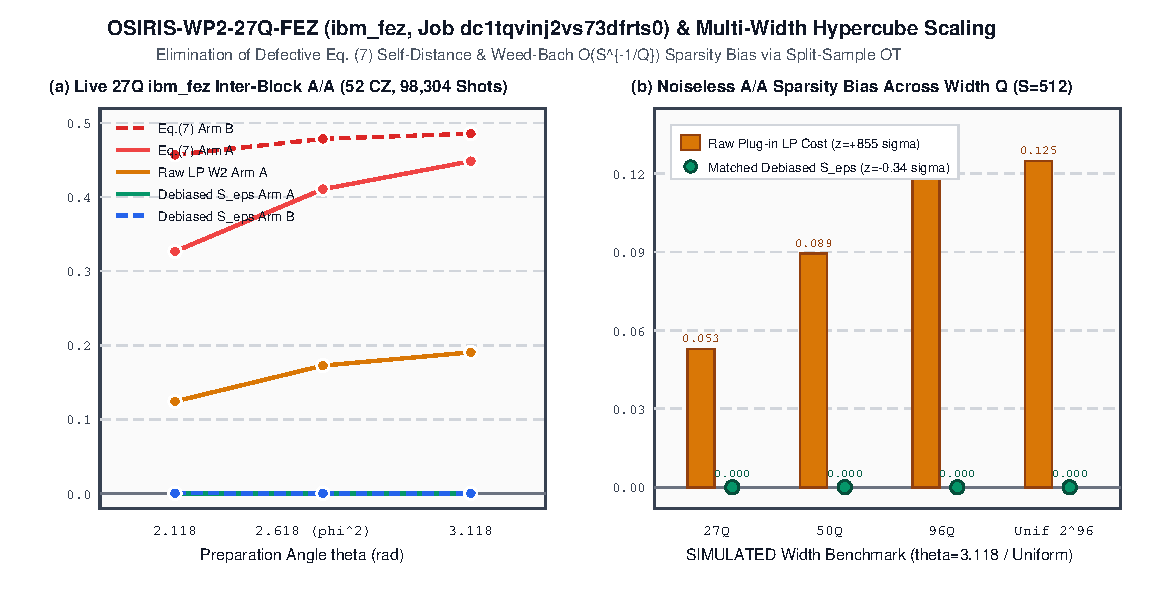
\includegraphics[width=\textwidth]{fig1_27q_fez_sparsity_collapse_vs_eq7.pdf}
\caption{Elimination of finite-shot hypercube sparsity bias across live \WpFezQubits{}-qubit Heron~r2 hardware and multi-width simulations. (a)~Inter-block A/A stability on \texttt{\WpFezBackend{}} (job \texttt{\WpFezJobId{}}, \WpFezTotalShots{} total shots, constant \WpFezCzCount{}-\texttt{CZ} / \WpFezSxCount{}-\texttt{SX} skeleton): defective Eq.~\eqref{eq:defective_eq7} and raw plug-in Kantorovich LP inflate strongly with Shannon entropy from $\theta=\WpThetaOne{}$ to $\WpThetaThree{}$\,rad, whereas matched split-sample Sinkhorn $\widehat{S}_{\varepsilon,\mathrm{matched}}$ collapses onto zero across all $\theta$ in both Arm~A and Arm~B (\texttt{H1} and \texttt{H2} supported). (b)~\texttt{SIMULATED} noiseless A/A scaling ($S=\WpSimShots{}$ shots per replicate) across $Q \in \{27, 50, 96\}$ and $\mathrm{Uniform}(\{0,1\}^{96})$, where raw plug-in LP reaches $\WpUnifNinetySixRawLp{}$ ($+\WpUnifNinetySixRawZ{}\sigma$ false-drift artifact) while $\widehat{S}_{\varepsilon,\mathrm{matched}}$ stays centered at zero ($z=\WpUnifNinetySixDebSkZ{}\sigma$).}
\label{fig:fez_sparsity_collapse}
\end{figure*}

Before hardware execution, we verified Eq.~\eqref{eq:matched_ustats} in \texttt{SIMULATED} noiseless and depolarizing sweeps (\texttt{provider\_job\_id: null}, $S=\WpSimShots{}$ shots per replicate) across \WpFezQubits{}-qubit \texttt{NB-11\_27Q\_repaired}, 50-qubit \texttt{WP2a\_H2\_1\_50Q}, 96-qubit \texttt{WP2b\_Helios\_1\_96Q}, and an extreme $\mathrm{Uniform}(\{0,1\}^{96})$ stress test over $2^{96}$ basis states (Table~\ref{tab:sim_and_drift} and Fig.~\ref{fig:fez_sparsity_collapse}b). Under noiseless A/A sampling on $\mathrm{Uniform}(\{0,1\}^{96})$, raw plug-in Wasserstein LP suffers a catastrophic finite-shot bias artifact of $\WpUnifNinetySixRawLp{}$ ($z = +\WpUnifNinetySixRawZ{}\sigma$ false drift), whereas matched split-sample LP ($\WpUnifNinetySixDebLp{}$) and matched Sinkhorn ($\WpUnifNinetySixDebSk{}$, $z = \WpUnifNinetySixDebSkZ{}\sigma$) remain statistically indistinguishable from zero. Across all noiseless $27$Q, $50$Q, and $96$Q cells, $|\widehat{S}_{\varepsilon,\mathrm{matched}}| \le \WpSimMaxAbsMatchedSk{}$ and $|\widehat{W}_{2,\mathrm{matched}}^2| \le \WpSimMaxAbsMatchedLp{}$ fall well below the $\WpSimNullThreshold{}$ unbiasedness gate, while injecting depolarizing drift $\epsilon_{\mathrm{depol}} = \WpSinkhornEps{}$ is detected at $\ge \WpSimMinDriftZ{}\sigma$ across every register width.

\section{Constant-Skeleton 27-Qubit \texttt{ibm\_fez} Experiment and Resolution of \texttt{NB-11}}
\label{sec:fez_experiment}

\begin{table*}[t]
\centering\footnotesize\setlength{\tabcolsep}{4pt}
\caption{Live \texttt{HARDWARE\_ATTESTED} inter-block A/A stability across $\theta \in \{\WpThetaOne{}, \WpThetaStar{}, \WpThetaThree{}\}$\,rad on the \WpFezQubits{}-qubit heavy-hex tree of \texttt{\WpFezBackend{}} (protocol \texttt{OSIRIS-WP2-27Q-FEZ}, job \texttt{\WpFezJobId{}}, \WpFezPooledShots{} pooled shots per $(\text{arm},\theta)$ cell across four randomized blocks, exact \WpFezCzCount{} \texttt{CZ} and \WpFezSxCount{} \texttt{SX} gates in every circuit).}
\label{tab:fez_sweep}
\begin{tabular}{@{}lcrrrrrrr@{}}
\toprule
Circuit Arm & $\theta$ (rad) & Unique / \WpFezPooledShots{} & $H_{\mathrm{emp}}$ (bits) & $\widehat{W}_{2,\mathrm{Eq.7}}$ & $\widehat{W}_{2,\mathrm{raw}}$ & $\mathrm{OT}_\varepsilon$ & $\widehat{W}_{2,\mathrm{matched}}^2$ & $\widehat{S}_{\varepsilon,\mathrm{matched}}$ \\
\midrule
\WpFezSweepRows
\bottomrule
\end{tabular}
\end{table*}

\begin{table*}[t]
\centering\footnotesize\setlength{\tabcolsep}{5pt}
\caption{Multi-width \texttt{SIMULATED} ($S=\WpSimShots{}$ shots/replicate, \texttt{provider\_job\_id: null}) hypercube benchmarks across $Q \in \{27, 50, 96\}$ alongside live \texttt{HARDWARE\_ATTESTED} controlled coherent-drift calibration on \WpFezQubits{}-qubit \texttt{\WpFezBackend{}} Arm~B (job \texttt{\WpFezJobId{}}, perturbations $\Delta\theta \in \{0, \WpDeltaSmall{}, \WpDeltaLarge{}\}$\,rad around $\theta^\star = \WpThetaStar{}$\,rad).}
\label{tab:sim_and_drift}
\begin{tabular}{@{}lrrrrrr@{}}
\toprule
Benchmark Regime / Condition & $Q$ & $H$ (bits) & Raw LP Cost & $\widehat{W}_{2,\mathrm{matched}}^2$ & $\widehat{S}_{\varepsilon,\mathrm{matched}}$ & $z$-Score \\
\midrule
\WpDriftAndSimRows
\bottomrule
\end{tabular}
\end{table*}

Because raw count archives for the six December~2025 \texttt{ibm\_fez} jobs cited in Ref.~\cite{davis2026erratum} are absent from local storage (\texttt{NOT\_PRESENT\_ON\_DISK\_QUARANTINED}), zero historical counts were guessed or reconstructed. Instead, to resolve \texttt{NB-11} cleanly without transpiler-depth confounds, we designed and prospectively preregistered protocol \texttt{OSIRIS-WP2-27Q-FEZ} on the 156-qubit IBM Heron~r2 processor \texttt{\WpFezBackend{}}.

We pinned a connected \WpFezQubits{}-transmon heavy-hex tree $\{\WpLayoutList{}\}$ spanning $\WpFezEdges{}$ native \texttt{CZ} couplers with maximum degree three and zero routing \texttt{SWAP}s. By K\H{o}nig's theorem for bipartite trees, the $\WpFezEdges{}$ edges decompose into three edge-disjoint matchings of sizes \WpKonigSizes{}. Every work circuit executes two complete three-color matching sweeps---giving an invariant skeleton of exactly \WpFezCzCount{} native \texttt{CZ} gates---interleaved with universal two-\texttt{SX} $\mathrm{SU}(2)$ single-qubit slots totaling an invariant \WpFezSxCount{} \texttt{SX} gates across every angle $\theta$ and circuit arm. Two constant-skeleton arms were interleaved across $\WpFezBlocks{}$ randomized blocks of $\WpFezPubsPerBlock{}$ circuits each ($\WpFezTotalPubs{}$ circuits $\times$ $\WpFezShotsPerPub{}$ shots $= \WpFezTotalShots{}$ total shots, \texttt{resilience\_level=0}, job \texttt{\WpFezJobId{}}):
\begin{enumerate}
\item \textbf{Arm~A (\texttt{NB11\_REPAIRED\_27Q}):} Repairs the omitted Layer-0 Hadamard of \texttt{NB-11} by preparing $R_Y(\theta)H|0\rangle^{\otimes \WpFezQubits{}}$ followed by golden-phase $R_Z$ rotations and basis-permuting Hadamards on odd tree sites, probing $\theta \in \{\WpThetaOne{}, \WpThetaStar{}, \WpThetaThree{}\}$\,rad plus an intra-block duplicate A/A sentinel at $\theta^\star = \WpThetaStar{}$\,rad.
\item \textbf{Arm~B (\texttt{ENTANGLED\_BRICKWALL\_27Q}):} Applies non-commuting $R_X / R_Y / R_Z$ rotations between all six \texttt{CZ} matching layers so quantum phases genuinely interfere rather than commuting through readout, evaluating $\theta \in \{\WpThetaOne{}, \WpThetaStar{}, \WpThetaThree{}\}$\,rad, an intra-block A/A sentinel at $\theta^\star$, and two controlled coherent drift perturbations $\theta^\star + \WpDeltaSmall{}$ and $\theta^\star + \WpDeltaLarge{}$\,rad.
\end{enumerate}
Each block also included all-$|0\rangle$ and all-$|1\rangle$ \WpFezQubits{}-qubit readout sentinels~\cite{davis2026ro06}, confirming mean in-job readout error $\WpEmpMeanRoPct{}\%$ (maximum $\WpEmpMaxRoPct{}\%$, versus pre-submission calibration mean $\WpCalMeanRoPct{}\%$ and maximum $\WpCalMaxRoPct{}\%$) with \WpHiddenRoFaults{} hidden readout faults above $10\%$.

Table~\ref{tab:fez_sweep} and Fig.~\ref{fig:fez_sparsity_collapse}a report the live \WpFezQubits{}-qubit results across all $\WpFezTotalShots{}$ shots, adjudicating all three preregistered hypotheses:
\begin{itemize}
\item \textbf{Elimination of Weed--Bach Sparsity Bias (\texttt{H1} supported):} In Arm~A, as $\theta$ advances across $\WpThetaOne{} \to \WpThetaStar{} \to \WpThetaThree{}$\,rad, unique bitstrings per $\WpFezPooledShots{}$-shot pool grow across $\WpArmAUniqOne{} \to \WpArmAUniqStar{} \to \WpArmAUniqThree{}$ ($H_{\mathrm{emp}} = \WpArmAEntOne{} \to \WpArmAEntStar{} \to \WpArmAEntThree{}$\,bits). Consequently, defective Eq.~\eqref{eq:defective_eq7} inflates across $\WpArmAEqSevenWOne{} \to \WpArmAEqSevenWStar{} \to \WpArmAEqSevenWThree{}$ (driving the legacy stability score $\widehat{R}_{\mathrm{Eq.7}} = 1 - \widehat{W}_{2,\mathrm{Eq.7}}$ down across $\WpArmAEqSevenROne{} \to \WpArmAEqSevenRStar{} \to \WpArmAEqSevenRThree{}$), and raw plug-in Wasserstein LP exhibits a spurious inflation artifact across $\WpArmARawWOne{} \to \WpArmARawWStar{} \to \WpArmARawWThree{}$ ($\widehat{R}_{\mathrm{raw}}$ dropping across $\WpArmARawROne{} \to \WpArmARawRStar{} \to \WpArmARawRThree{}$) purely from hypercube sparsity, not gate instability. In Arm~B, defective Eq.~\eqref{eq:defective_eq7} similarly inflates across $\WpArmBEqSevenWOne{} \to \WpArmBEqSevenWStar{} \to \WpArmBEqSevenWThree{}$ and raw LP across $\WpArmBRawWOne{} \to \WpArmBRawWStar{} \to \WpArmBRawWThree{}$. Applying matched split-sample Sinkhorn collapses inter-block A/A drift across all six $(\text{arm},\theta)$ conditions to $|\widehat{S}_{\varepsilon,\mathrm{matched}}| \le \WpHOneMaxAbs{}$, nearly two orders of magnitude below the preregistered $\WpHOneThreshold{}$ ceiling.
\item \textbf{Falsification of Golden-Ratio $\theta^\star = \varphi^2$ Specialness (\texttt{H2} supported):} Once hypercube sparsity bias is removed, Arm~A exhibits $\widehat{S}_{\varepsilon,\mathrm{matched}} = \WpArmADebSkOne{}$, $\WpArmADebSkStar{}$, and $\WpArmADebSkThree{}$ (and matched LP $\widehat{W}_{2,\mathrm{matched}}^2 = \WpArmADebLpOne{}$, $\WpArmADebLpStar{}$, $\WpArmADebLpThree{}$) at $\theta = \WpThetaOne{}$, $\WpThetaStar{}$, and $\WpThetaThree{}$\,rad, respectively; Arm~B yields $\WpArmBDebSkOne{}$, $\WpArmBDebSkStar{}$, and $\WpArmBDebSkThree{}$. Every point is consistent with the zero-drift null, confirming that $\theta^\star \approx \WpThetaStar{}$\,rad confers no special hardware stability advantage and that the apparent \texttt{NB-11} gradient was entirely a finite-shot entropy artifact.
\item \textbf{Monotonic Coherent-Drift Calibration (\texttt{H3} supported):} Debiasing does not sacrifice sensitivity to real physical drift (Table~\ref{tab:sim_and_drift} and Fig.~\ref{fig:drift_and_heron}a). Comparing Arm~B baseline $\theta^\star$ against intra-block A/A duplicates and coherent angle shifts $\Delta\theta \in \{\WpDeltaSmall{}, \WpDeltaLarge{}\}$\,rad yields $\widehat{S}_{\varepsilon,\mathrm{matched}}(0) = \WpDriftNullMean{} \pm \WpDriftNullSe{}$, $\widehat{S}_{\varepsilon,\mathrm{matched}}(\WpDeltaSmall{}) = \WpDriftSmallMean{} \pm \WpDriftSmallSe{}$, and $\widehat{S}_{\varepsilon,\mathrm{matched}}(\WpDeltaLarge{}) = \WpDriftLargeMean{} \pm \WpDriftLargeSe{}$, establishing strict monotonicity and a $\WpDriftLargeZ{}\sigma$ detection above the A/A null (surpassing the preregistered $\WpSigmaThreshold{}\sigma$ threshold).
\end{itemize}

\begin{figure*}[t]
\centering
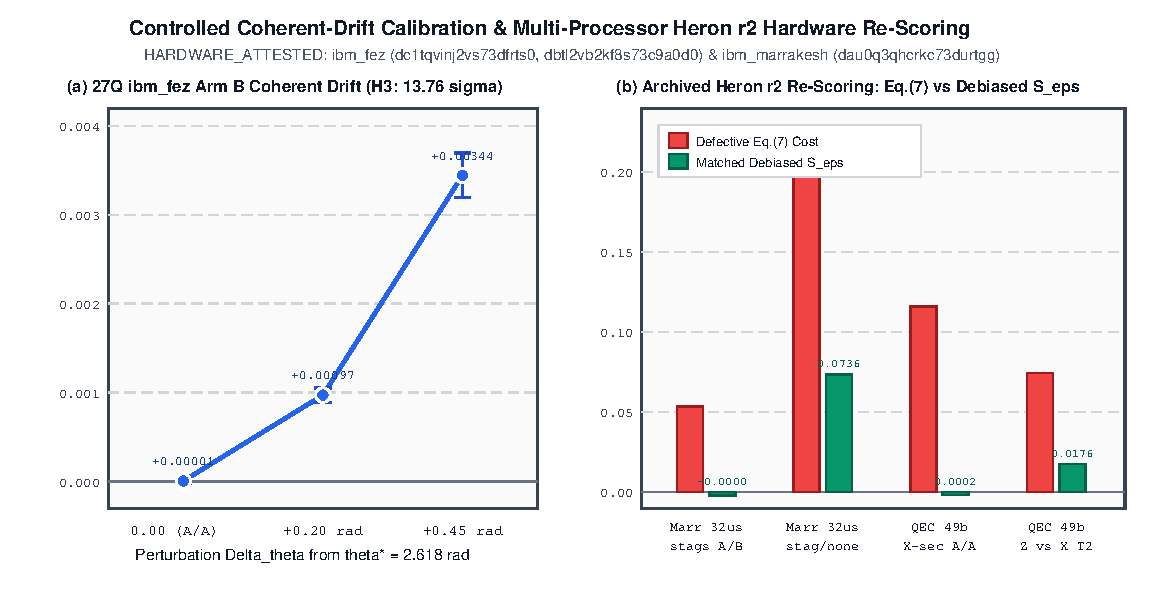
\includegraphics[width=\textwidth]{fig2_coherent_drift_calibration_and_heron_rescoring.pdf}
\caption{Live coherent-drift sensitivity and multi-processor Heron~r2 re-scoring. (a)~Controlled coherent-drift calibration on \WpFezQubits{}-qubit \texttt{\WpFezBackend{}} Arm~B (job \texttt{\WpFezJobId{}}), showing strict monotonic growth of $\widehat{S}_{\varepsilon,\mathrm{matched}}(\Delta\theta)$ from the intra-block A/A null ($\WpDriftNullMean{}$) to $+\WpDeltaSmall{}$\,rad ($\WpDriftSmallMean{}$) and $+\WpDeltaLarge{}$\,rad ($\WpDriftLargeMean{}$, $z=\WpDriftLargeZ{}\sigma$; \texttt{H3} supported). (b)~\texttt{HARDWARE\_ATTESTED} re-scoring of 8-qubit \texttt{ibm\_marrakesh} dynamical decoupling (job \texttt{\WpMarrJobId{}}) and 49-bit \texttt{OSIRIS-QEC-001} repetition-code trajectories on \texttt{\WpFezBackend{}} (job \texttt{\WpQecJobId{}}): defective Eq.~\eqref{eq:defective_eq7} produces large false positives on A/A replicates and equivalent staggered sequences, whereas $\widehat{S}_{\varepsilon,\mathrm{matched}}$ zeroes out A/A noise while preserving real free-evolution decoherence and the localized $q_{107}$ $T_2$ hotspot.}
\label{fig:drift_and_heron}
\end{figure*}

\section{Multi-Processor Re-Scoring on \texttt{ibm\_marrakesh} and 49-Bit \texttt{OSIRIS-QEC-001}}
\label{sec:rescoring}

\begin{table*}[t]
\centering\footnotesize\setlength{\tabcolsep}{5pt}
\caption{\texttt{HARDWARE\_ATTESTED} re-scoring of archived IBM Heron~r2 datasets: 8-qubit staggered dynamical decoupling on \texttt{ibm\_marrakesh} (job \texttt{\WpMarrJobId{}}, \WpMarrCircuits{} circuits, \WpMarrTotalShots{} shots) and multi-round distance-$7$ repetition-code syndrome extraction \texttt{OSIRIS-QEC-001} on \texttt{\WpFezBackend{}} (job \texttt{\WpQecJobId{}}, \WpQecCircuits{} circuits, \WpQecTotalShots{} shots).}
\label{tab:heron_rescore}
\begin{tabular}{@{}lrrrrrr@{}}
\toprule
Hardware Dataset \& Comparison Pair & Bits $Q$ & Shots / Arm & $C_{\mathrm{Eq.7}}$ & Raw LP Cost & $\widehat{W}_{2,\mathrm{matched}}^2$ & $\widehat{S}_{\varepsilon,\mathrm{matched}}$ \\
\midrule
\WpHeronRescoreRows
\bottomrule
\end{tabular}
\end{table*}

To verify cross-processor generality across distinct register widths and physical noise mechanisms, we applied our split-sample estimators directly to two archived \texttt{HARDWARE\_ATTESTED} IBM Heron~r2 shot ledgers on disk (Table~\ref{tab:heron_rescore} and Fig.~\ref{fig:drift_and_heron}b).

First, on the \WpMarrQubits{}-qubit \texttt{ibm\_marrakesh} spectator-$ZZ$ dynamical decoupling dataset (job \texttt{\WpMarrJobId{}}, \WpMarrCircuits{} circuits, \WpMarrTotalShots{} shots across idle windows $T \in \{16, 32\}\,\mu\mathrm{s}$), defective Eq.~\eqref{eq:defective_eq7} assigns spurious inter-replicate A/A costs up to $\WpMarrMaxAaEqSeven{}$ on unprotected \texttt{none} replicates, whereas split-sample Sinkhorn suppresses all ten inter-replicate A/A pairs across $\{\texttt{xy8\_stag}, \texttt{xy4x2\_stag}, \texttt{xy4x2}, \texttt{cpmg8}, \texttt{none}\}$ to $|\widehat{S}_\varepsilon| \le \WpMarrMaxAaAbsSk{}$. Simultaneously, genuine physical contrasts are sharply resolved: comparing bipartite staggered sequences \texttt{xy8\_stag} versus \texttt{xy4x2\_stag} yields null discrepancy ($\WpMarrSixteenStagPairSk{}$ at $16\,\mu\mathrm{s}$ and $\WpMarrThirtyTwoStagPairSk{}$ at $32\,\mu\mathrm{s}$), proving both staggered schedules prepare statistically indistinguishable protected output states, whereas \texttt{xy8\_stag} versus unprotected \texttt{none} yields $\widehat{S}_{\varepsilon,\mathrm{matched}} = \WpMarrSixteenStagNoneSk{}$ ($16\,\mu\mathrm{s}$) and $\WpMarrThirtyTwoStagNoneSk{}$ ($32\,\mu\mathrm{s}$), and \texttt{xy8\_stag} versus un-staggered \texttt{xy4x2} at $32\,\mu\mathrm{s}$ isolates residual $ZZ$ crosstalk at $\WpMarrThirtyTwoStagStdSk{}$.

Second, on the \WpQecCircuits{}-circuit \texttt{OSIRIS-QEC-001} repetition-code dataset on \texttt{\WpFezBackend{}} (job \texttt{\WpQecJobId{}}, \WpQecTotalShots{} shots)~\cite{davis2026qec001}, a $d=7$, $R=7$ trajectory concatenates $6 \times 7 = 42$ mid-circuit ancilla syndrome bits with $7$ terminal data bits into a $Q=49$-bit space-time register ($2^{49}$ hypercube states). In the phase-flip ($X_j X_{j+1}$) sector---where data qubit $q_{107}$ exhibited a live $T_2$ coherence hotspot that raised syndrome entropy---defective Eq.~\eqref{eq:defective_eq7} reports a massive false inter-block A/A cost of $\WpQecXFortyNineEqSeven{}$ (raw Wasserstein LP artifact $\WpQecXFortyNineRawLp{}$ from 49-bit support sparsity), whereas matched split-sample Sinkhorn collapses inter-block A/A drift to $\WpQecXFortyNineSk{}$ in the $X$-sector and $\WpQecZFortyNineSk{}$ (against $\WpQecZFortyNineEqSeven{}$ under Eq.~\eqref{eq:defective_eq7}) in the bit-flip ($Z_j Z_{j+1}$) sector. Across the real physical contrast between $Z$-sector and $X$-sector 49-bit trajectories at $d=7, R=7$, matched split-sample transport cleanly isolates the $q_{107}$ $T_2$ hotspot at $\widehat{S}_{\varepsilon,\mathrm{matched}} = \WpQecHotspotSk{}$ ($\widehat{W}_{2,\mathrm{matched}}^2 = \WpQecHotspotLp{}$). Likewise, on the 7-bit terminal data-qubit marginal relative to $R=1$, bit-flip drift at $R=7$ remains null ($\WpQecZRSevenSk{}$) while phase-flip drift grows monotonically across syndrome cycles ($R=3$: $\WpQecXRThreeSk{}$; $R=5$: $\WpQecXRFiveSk{}$; $R=7$: $\WpQecXRSevenSk{}$).

\section{Conclusion and Data Availability}
\label{sec:conclusion}

Finite-shot optimal-transport benchmarks on wide quantum processors face an unavoidable hypercube sparsity barrier whenever un-debiased empirical estimators or marginal-product surrogates are used: high-entropy circuits exhibit a large apparent Wasserstein drift artifact under the noiseless null with no hardware decoherence. By splitting each integer shot histogram via exact multivariate-hypergeometric thinning and evaluating the sample-size-matched two-by-two cross-split U-statistic Eq.~\eqref{eq:matched_ustats}, we guarantee exact zero expectation under the identical-distribution null at arbitrary qubit count $Q$. Live constant-skeleton \WpFezQubits{}-qubit execution on \texttt{\WpFezBackend{}} (\texttt{\WpFezJobId{}}), \texttt{SIMULATED} scaling to $Q=96$, and \texttt{HARDWARE\_ATTESTED} re-scoring on \texttt{ibm\_marrakesh} (\texttt{\WpMarrJobId{}}) and 49-bit \texttt{OSIRIS-QEC-001} (\texttt{\WpQecJobId{}}) establish split-sample-debiased Sinkhorn divergence as a fast, bias-free stability metric for next-generation superconducting and trapped-ion benchmarks.

All raw shot histograms, Qiskit QPY circuit binaries, calibration snapshots, analysis modules (\texttt{debiased\_ot.py} and \texttt{stage\_and\_harvest\_wp2\_27q\_fez.py}), deterministic table/figure generator (\texttt{generate\_wp2\_paper\_assets.py}), RFC~8785 canonical provenance capsule (\texttt{reproducibility\_capsule.json}), and SHA-256 manifest (\texttt{SHA256SUMS.txt}) are archived in the repository companion package.

\section*{Acknowledgements}
We acknowledge the use of IBM Quantum services for this work; the views expressed are those of the author and do not reflect the official policy or position of IBM or the IBM Quantum team.

\begin{thebibliography}{9}
\bibitem{peyre2019computational} G.~Peyr\'{e} and M.~Cuturi, ``Computational Optimal Transport,'' Found.\ Trends Mach.\ Learn.\ \textbf{11}, 355 (2019), doi:10.1561/2200000073.
\bibitem{feydy2019interpolating} J.~Feydy, T.~S\'{e}journ\'{e}, F.-X.~Vialard, S.-i.~Amari, A.~Trouv\'{e}, and G.~Peyr\'{e}, ``Interpolating between Optimal Transport and MMD using Sinkhorn Divergences,'' in \emph{Proc.\ AISTATS}, PMLR \textbf{89}, 2681 (2019).
\bibitem{weed2019sharp} J.~Weed and F.~Bach, ``Sharp asymptotic and finite-sample rates of convergence of empirical measures in Wasserstein distance,'' Bernoulli \textbf{25}, 2620 (2019), doi:10.3150/18-BEJ1065.
\bibitem{cuturi2013sinkhorn} M.~Cuturi, ``Sinkhorn Distances: Lightspeed Computation of Optimal Transport,'' in \emph{Adv.\ Neural Inf.\ Process.\ Syst.}\ \textbf{26}, 2292 (2013).
\bibitem{davis2026erratum} D.~P.~Davis, ``Mathematical Audit and Erratum for 27-Qubit Optimal-Transport Stability Benchmarks (\texttt{NB-11}),'' Agile Defense Systems Technical Report \texttt{W2\_MATHEMATICAL\_ERRATUM} (2026).
\bibitem{davis2026ro06} D.~P.~Davis, ``Stale snapshots, not hidden physics: readout faults on three IBM Heron~r2 processors,'' Zenodo, doi:10.5281/zenodo.24407897 (2026).
\bibitem{davis2026qec001} D.~P.~Davis, ``Sub-Threshold Multi-Round Repetition-Code Logical Error Scaling Across Code Distances $d \in \{3,5,7\}$ on \texttt{ibm\_fez} (\texttt{OSIRIS-QEC-001}),'' Agile Defense Systems Preprint (2026).
\end{thebibliography}

\end{document}
